\chapter{Alineacion de imagenes}
\label{capitulo3}
\lhead{Capítulo 3. \emph{Alineacion de imagenes}}

\section{Introduccion}

Introduccion

\begin{figure}[H]
	\centering
	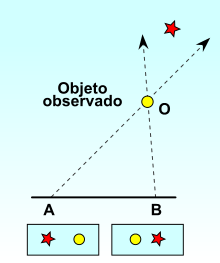
\includegraphics[width=0.85\textwidth]{paralaje1}
	\caption[Paralaje - Efectos en el cambio de punto de vista]{Efectos en el cambio del punto de vista.}
	\label{imagen:paralaje}
\end{figure}

Desde el punto de vista \textbf{A}, se observa la estrella a la izquierda del circulo. Mientras que desde le punto \textbf{B} la estrella es observada a la derecha del circulo.

\section{Transformaciones geometricas}
Prueba

\section{Generacion de sub-mosaicos}
Prueba

\subsection{Seleccion de imagen de referencia}
Prueba

\subsection{Matriz de homografia promedio}
Prueba

\section{Coreccion euclideana}
Prueba

\section{Resumen}
Resumen



\section{Algoritmos (temporal)}
\begin{algorithm}[H] %or another one check
	\caption{Calculo de matriz de homografia promedio}
	\SetAlgoLined
		   
	\While{no se alcanza el maximo de iteraciones}{
		seleccionar 4 puntos aleatorios del primer sub-mosaico\;
		seleccionar los 4 puntos correspondientes en el segundo sub-mosaico\;
		calcular el punto medio para cada par de puntos correspondientes\;
		calcular la transformacion desde los puntos del primer sub-mosaico hasta los puntos medios\;
		aplicar transformacion en el primer sub-mosaico\;
		calcular error de distorsión en el primer sub-mosaico\;
		\eIf{el error es menor que el mas bajo obtenido}{
			guardar el error como el mas bajo\;
			guardar la matriz de transformación como la mejor\;
			}{
			restaurar valores del primer sub-mosaico\;
		}
	}
\end{algorithm}

\begin{algorithm}[H] %or another one check
	\caption{Encontrar matriz de transformacion}
	\SetAlgoLined
	 $I_{i+1}$ $\equiv$ Imagen nueva\;
	 $I_{i}$ $\equiv$ ultima imagen anadida al mosaico\;
	 $V_{i}$ $\equiv$ vecinos de $I_{i}$\;
	\While{puntos emparejados $\ge$ 4}{
		 Emparejar puntos de $I_{i+1}$ con $I_{i}$\;
		 \If{$I_{i}$ tiene vecinos}{
			 	\ForEach {vecinos de $I_{i}$}{
			 		Emparejar puntos de $I_{i+1}$ con $V_{i}$\;
			 	}
		 }
		 descartar malos emparejamientos;
		 aplicar busqueda sectorizada;
		 \If{puntos totales emparejados $\le$ 3}{
			 	modificar criterio para descartar\;
			 	\If{criterio para descartar llega al minimo}{
			 		terminar \tcp*{no es posible emparejar imagen}
			 	}
		 }
	}
\end{algorithm}



